\documentclass[9pt]{beamer}
\usepackage[utf8]{inputenc}
\usepackage{txfonts}
\usepackage[english]{babel}
\usepackage{xcolor}
\usepackage{soul}
% \usepackage{epigraph}
% \usepackage{cmll}
% \usepackage{pgfcore}
% \usepackage{graphicx}
\usetheme{CambridgeUS}
\usecolortheme{beaver}

\setbeamertemplate{headline}{}
% \setbeamertemplate{frametitle}{\insertframetitle}
\setbeamertemplate{navigation symbols}{}

\setbeamertemplate{itemize item}{\scriptsize\raise1.25pt\hbox{\donotcoloroutermaths$\blacktriangleright$}}
\setbeamertemplate{itemize subitem}{\tiny\raise1.5pt\hbox{\donotcoloroutermaths$\blacktriangleright$}}
\setbeamertemplate{itemize subsubitem}{\tiny\raise1.5pt\hbox{\donotcoloroutermaths$\blacktriangleright$}}
\setbeamertemplate{enumerate item}{\insertenumlabel.}
\setbeamertemplate{enumerate subitem}{\insertenumlabel.\insertsubenumlabel}
\setbeamertemplate{enumerate subsubitem}{\insertenumlabel.\insertsubenumlabel.\insertsubsubenumlabel}
\setbeamertemplate{enumerate mini template}{\insertenumlabel}

% \setbeamertemplate{itemize items}[square]
% \setbeamertemplate{items}[square]



\newcommand{\bluemph}[1]{\structure{\emph{#1}}}
\newcommand{\redemph}[1]{\alert{\emph{#1}}}
\newcommand{\bluebf}[1]{\structure{\textbf{#1}}}
\newcommand{\redbf}[1]{\alert{\textbf{#1}}}

\newcommand\denote[1]{\llbracket #1 \rrbracket}
\newcommand\fesi{Fe-Si}

%  Structure
\newenvironment{remark}{\footnotesize \begin{description}\item[\emph{Remark}:]}{\end{description}}

\title{Formal verification of hardware synthesis}%
\author{Thomas Braibant \and Adam Chlipala}
\institute[UoG, MIT]{University of Grenoble \and MIT CSAIL}
\date[08/2012]{Coq Workshop 2012}

\setbeamercovered{transparent}
\setbeamerfont{frametitle}{size={\normalsize}}

% \usepackage[T1]{fontenc}
\usepackage{amsmath}
\usepackage{amssymb}
\usepackage{amsthm}
\usepackage{mathpartir}

\usepackage{listings}
\usepackage{graphicx}
\definecolor{ltblue}{rgb}{0,0.4,0.4}
\definecolor{dkblue}{rgb}{0,0.1,0.6}
\definecolor{dkgreen}{rgb}{0,0.4,0}
\definecolor{dkviolet}{rgb}{0.3,0,0.5}
\definecolor{dkred}{rgb}{0.5,0,0}
\usepackage{lstcoq}
\usepackage{lstocaml}
\newenvironment{twolistings}%
{\noindent\begin{tabular*}{\linewidth}{@{}c@{\extracolsep{\fill}}c@{}}}%
{\end{tabular*}}

% \AtBeginSection[]
% {
%    \begin{frame}
%        \frametitle{Outline}
%        \tableofcontents[currentsection,currentsubsection]
%    \end{frame}
% }

\begin{document}
% \newcommand \blue[1]{{\color{red!80!black}{#1}}}
\newcommand \orange[1]{{\color{orange}{#1}}}
% \newcommand \red[1]{{\color{red}{#1}}}
% \newcommand \grey[1]{{\color{gray}{#1}}}
% \newcommand \green[1]{{\color{violet}{#1}}}
% \newcommand \white[1]{{\color{white}{#1}}}

\newcommand\parenthesis[1] {
  \begin{flushright}
    {\scriptsize \redemph{{{{ #1}}}}}
  \end{flushright}

}

\begin{frame}
  \center 
  \titlepage
\end{frame} 

%%%%%%%%%%%%%%%%%%%%%%%%%%%%%%%%%%%%%% 
\begin{frame}
  \frametitle{Context: formal verification of hardware}
  
  \begin{itemize}
  % \item  Formally verified everything:
  %   \begin{itemize}
  %   \item Compilers (CompCert [2006])
  %   \item Operating Systems (Gypsy [1989]; seL4 [2009])
  %   \item Static analysers
  %   \item \alert<2->{Hardware}
  %   \end{itemize}
  
  % \pause

  \item Verifying hardware with theorem provers:
    \begin{itemize}
    \item many \emph{shallow-embeddings} of hardware description languages (ACL2 , HOL, PVS)
      % ACL2 :DE2
      % Hol : Experience with embedding hardware description languages in HOL (1992)
      % PVS : Bluespec
    \item many \emph{shallow-embeddings} of hardware designs (ACL2, HOL, PVS, Coq) 
      \begin{itemize}
      \item[-] Floating-point operations verified at AMD using ACL2 
      \item[-] VAMP [2003]  (a pipelined micro-processor verified in PVS)
      \end{itemize}
    \item high-level formalization of the ARM architecture in HOL
    \item ...
    \end{itemize}

    \pause
    
    % This verification does not match what is really done
  \item Industry shifts toward \alert{hardware synthesis}: 
    \begin{itemize}
    \item generates low-level code (RTL) from high-level HDLs
    \item argue (in)formally that this synthesis is correct
    \end{itemize}
    \parenthesis{Bluespec, Esterel, Lustre, \dots}
  \end{itemize}
\end{frame}

%%%%%%%%%%%%%%%%%%%%%%%%%%%%%%%%%%%%%% 
\begin{frame}
  \frametitle{This project}
  \framesubtitle{on-going work}
  \begin{itemize}
  \item  Investigate hardware synthesis in Coq
    
    \begin{center}
      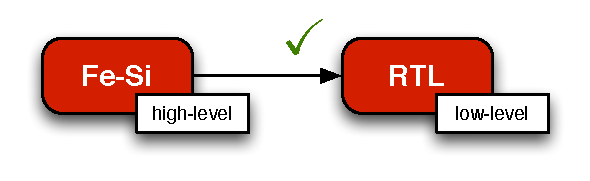
\includegraphics[height= 2cm ]{figs/compilation.pdf}
    \end{center}
    \pause
    
  \item Source language: \alert{\fesi{}} (Featherweight Synthesis)
    \begin{itemize}
    \item Stripped down and simplified version of \alert{Bluespec} 
    \item Semantics based on ``guarded atomic actions'' (with a flavour of transactional memory)
    \end{itemize}
    
    \pause
    
  \item Target language: RTL
    \begin{itemize}
    \item Combinational logic and next-state assignments for registers
    \item No currents, no delays, single-clock
    \end{itemize}
    
    \pause
    
  \item We define \emph{deep-embeddings}
    \begin{itemize}
    \item Define data-structures to represent programs
    \item Define what is a program's semantics (via an interpretation function) 
    \end{itemize}
  \item Use \alert{parametric higher-order abstract syntax} (PHOAS) to deal with binders
  \end{itemize}
\end{frame}


\defverbatim[colored]\phoasprimer{
}
\begin{frame}[fragile]
  \frametitle{A PHOAS primer}
  \begin{itemize}
  \item Use Coq bindings to represent the bindings of the object language.
    \newcommand\arrow{\ulcorner \to \urcorner}
\begin{coq}
Section t. 
  Variable var: T -> Type.
  
  Inductive term : T -> Type :=
  | Var: forall t, var t -> term t
  | Abs: forall $\alpha$ $\beta$, (var $\alpha$ -> term $\beta$) -> term ($\alpha$ $\arrow$ $\beta$)
  | App: ...
End t. 

Definition Term := forall (var: T -> Type), term var. 

Example K $\alpha$ $\beta$ : Term ($\alpha~\arrow{}~\beta{}~\arrow{}~\alpha$):= fun V =>
$\quad$Abs (fun x => Abs (fun y => Var x)).
\end{coq}

\pause

\item An \alert{intrinsic approach} (strongly typed syntax vs. syntax + typing judgement)
\item Program transformations are easier to implement (and prove!) 
  \parenthesis{with one caveat}
\end{itemize}
\end{frame}
% \begin{frame}[fragile]
%   \frametitle{A PHOAS primer}
%   \framesubtitle{Face-off with Dependent de Bruijn indices}
%   \begin{columns}
%     \column{0.07 \linewidth}
%     \column{0.5 \linewidth}
% \newcommand\env{\Gamma}
% \begin{coq}
% Inductive var : list T -> T -> Type :=
% | 0 : forall $\env$ t , var (t::$\env$) t
% | S : forall $\env$ t u , var $\env$ u -> var (t::$\env$) u. 

% Inductive term : list T -> T -> Type :=
% | Var: forall $\env$ t, var $\env$ t -> term $\env$ t
% | Abs: forall $\env$ $\alpha$ $\beta$, term ($\alpha$:: $\env$) $\beta$ -> 
%            term $\env$ ($\alpha$ $\ulcorner \to \urcorner$ $\beta$)
% | App: ...  

% Example K := 
% $\quad$Abs (Abs (Var (S 0))).
% \end{coq}
%     \column{0.5 \linewidth}
% \only<2->{\phoasprimer}
%   \end{columns}
%   \begin{itemize}
%   \item<3> Two alternative  \alert{intrinsic approaches}
%     \begin{itemize}
%     \item strongly typed syntax
%     \item alternative to syntax + typing judgement
%     \end{itemize}
%   \end{itemize}
% \end{frame}

%%%%%%%%%%%%%%%%%%%%%%%%%%%%%%%%%%%%%% 

\begin{frame}
  \frametitle{Outline}       
  \tableofcontents  
\end{frame}

%%%%%%%%%%%%%%%%%%%%%%%%%%%%%%%%%%%%%% 

%%%%%%%%%%%%%%%%%%%%%%%%%%%%%%%%%%%%%% 

\section{A glimpse of the languages and the compiler}
\begin{frame}[fragile]
  \frametitle{\fesi{} in a nutshell}

  \fesi{} programs:
  \begin{itemize}
  \item update a set of \alert{memory elements} $\Phi$;
    \\
    \parenthesis{registers, register files, fifos, \dots}
  \item are based on \alert{guarded atomic actions} 
    \\
    \begin{center}
    \coqe{do n <- !x + 1; (y := 1; assert (n = 0)) orElse (y := 2)}      
    \end{center}
  \item are endowed with a (simple) \alert{synchronous semantics}
    \\
    \begin{center}
    \coqe{do n <- !x; x := n + 1; do m <- !x; assert (n = m)}
    \end{center}
  \end{itemize}
\end{frame}

\begin{frame}[fragile]
  \frametitle{\fesi{} in a nutshell}
  \begin{columns}
\column{0.1\linewidth}

\column{0.6 \linewidth}
\begin{coq}
Variable V: T -> Type. 
Inductive $\mathbb A$: T -> Type:=
| Return: forall t, expr t -> $\mathbb A$ t
| Bind: forall t u,  $\mathbb A$  t -> (V t -> $\mathbb A$ u) -> $\mathbb A$ u

(** effects **)
| Primitive: ... 

(** control-flow **)
| OrElse: forall t, $\mathbb A$ t -> $\mathbb A$ t -> $\mathbb A$ t.
| Assert: expr Tbool -> $\mathbb A$ Tunit\end{coq}
    \end{columns}


\begin{itemize}
\item Expressions are side-effects free. 
\item Primitives are operations on memory elements (dependent on $\Phi$)
\item 
  \begin{coq}
Definition Eval $\Phi$ t (a: forall V, $\mathbb A$ V t): $\denote\Phi$ -> option ($\denote{\tt t}$ * $\denote\Phi$).
\end{coq}
\end{itemize}

\end{frame}
%%%%%%%%%%%%%%%%%%%%%%%%%%%%%%%%%%%%%% 
\begin{frame}[fragile]
  \frametitle{RTL in a nutshell}
  \begin{columns}
    \column{0.5 \textwidth}
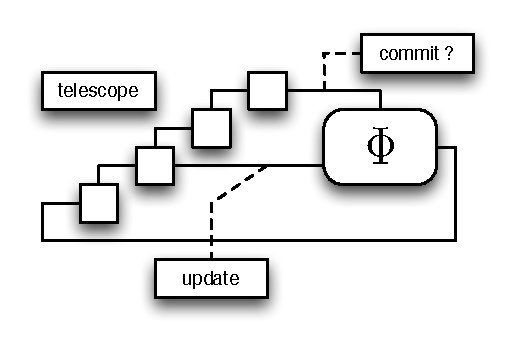
\includegraphics[width=5cm]{figs/rtl.pdf}
    
    \column{0.5 \textwidth}
    \begin{coq}
Variable V: T -> Type.       

Inductive $\mathbb T$ (A: Type): Type:=
| Bind: forall arg, expr arg -> (V arg -> $\mathbb T$ A) -> $\mathbb T$ A
| End: A -> $\mathbb T$ A.

Inductive $\mathbb E$: memory -> Type:=
| write: forall t,  V t -> V Tbool -> $\mathbb E$ (R t)
| ...

Definition block t:=
  $\mathbb T$ (V Tbool  * V t  * DList.T (option $\circ$ $\mathbb E$) $\Phi$). 
\end{coq}
  \end{columns}


\begin{itemize}
\item Simple synchronous semantics 
  \begin{coq}
Definition Eval $\Phi$ t (a: forall V, block V t): $\denote\Phi$ -> option ($\denote{\tt t}$ * $\denote\Phi$).
\end{coq}
\end{itemize} 
\end{frame}
%%%%%%%%%%%%%%%%%%%%%%%%%%%%%%%%%%%%%% 

\defverbatim[colored]\firstpass{
\begin{ocaml}
x0 <-  ! r1;
x1 <- x0 <> 0;
x2 <-  !r2;
x3 <- x0 - 1;
x4 <- x2 + 1;
x5 <-  !r2;
x6 <- x6;
begin 
  if x1 then (r1 := x3; r2 := x4);
  if  !x1 then (r1 := x6)
end
\end{ocaml}} 

\defverbatim[colored]\secondpass{
\begin{ocaml}
x0   <-  ! r1;
x1   <- x0 <> 0;
x2   <-  ! r2;
x3   <- x0 - 1;
x4   <- x2 + 1;
x5   <-  ! r2;
x6   <- x5;
x8   <- x1;
x9   <- x1;
x10 <- not x1;
x11 <- x8 || x10;
x12 <- x8 ?  x3 : x6;
begin 
  r1 := x12 when x11;
  r2 := x4 when x9
end
\end{ocaml}} 

\defverbatim[colored]\thirdpass{
\begin{ocaml}
x0   <- !r1 
x1   <- 0;
x2   <- x0 = x1;
x3   <- not x2;
x4   <- !r2;
x5   <- 1;
x6   <- x0 - x5;
x7   <- x4 + x5;
x8   <- !r2;
x9   <- not x3;
x10 <- x3 || x9
x11 <-x3 ? x6 : x8
begin
  r1 := x11 when x10;
  r2 := x8 when x3
end
\end{ocaml}}

\defverbatim[colored]\finalpass{
\begin{ocaml}
x0   <- !r1 
x1   <- 0;
x2   <- x0 = x1;
x3   <- not x2;
x4   <- !r2;
x5   <- 1;
x6   <- x0 - x5;
x7   <- x4 + x5;
x8   <-x3 ? x6 : x4
begin
  r1 := x8 when true;
  r2 := x4 when x3
end
\end{ocaml}}

\begin{frame}[fragile]
  \frametitle{Compiling \fesi{} to RTL}
  
Running example:
\begin{coq}
do x <- ! r1;if (x <> 0) then {do y <- !r2; r1 := x - 1; r2 := y + 1} else { y <- !r2; r1 := y}
\end{coq}
 
\pause
\begin{columns}
\column{0.1 \textwidth}  
\column{0.5 \textwidth}  
\begin{enumerate}
\item<+-> Pull out all bindings (that is, ANF)
\item<+-> Push down the nested conditions
\item<+-> Perform CSE (in 3-address code)
\item<+-> WIP: Boolean simplification
\end{enumerate}
\column{0.5 \textwidth}  
\only<2>{\firstpass}
\only<3>{\secondpass}
\only<4>{\thirdpass}
\only<5>{\finalpass}
\end{columns}
\end{frame}

%%%%%%%%%%%%%%%%%%%%%%%%%%%%%%%%%%%%%% 
\begin{frame}[fragile]
  \frametitle{PHOAS in action}

  \begin{itemize}
  \item<+-> (Temporary) final result
\begin{coq}
Definition Compile $\Phi$ t  (a : forall V, $\mathbb A$ $\Phi$ V t) : forall V, block V $\Phi$ t :=
  let x := Flat.Compile $\Phi$ t (Push.Compile $\Phi$  t (Pull.Compile $\Phi$  t a)) in
  CSE.Compile $\Phi$ t x.
\end{coq}

\begin{coq}
Theorem Compile_correct $\Phi$ t a :
  let x := Flat.Compile $\Phi$ t (Push.Compile $\Phi$  t (Pull.Compile $\Phi$  t a)) in
  WF $\Phi$ t x -> forall (st : $\denote\Phi$),  Eval $\Phi$ t (CSE.Compile $\Phi$ t x) st = Eval $\Phi$ t a st. 
\end{coq}

\item<+-> No need to prove lemmas about substitutions!
\item<+-> What about \coqe{WF $\Phi$ t x} ? 
\end{itemize}
\end{frame}

\begin{frame}[fragile]
  \frametitle{Well-formedness}

  \begin{itemize}
  \item   \coqe{WF $\Phi$ t x} states that \coqe{x} is  parametric w.r.t. the instantiation of \coqe{V}. 
  \item  We may:
    \begin{itemize}
    \item posit \coqe{forall x, WF $\Phi$ t x} as an axiom (informed
      parties think that this is consistent with Coq)
    \item or define what is \coqe{WF} for each language, prove that compilation preserves \coqe{WF} and prove that each starting program is \coqe{WF} 
    \item or generates \coqe{WF $\Phi$ t x} as a \alert{proof-obligation}, and discharge it using tactics
    \end{itemize}
  \end{itemize}
\end{frame}
%%%%%%%%%%%%%%%%%%%%%%%%%%%%%%%%%%%%%% 
\section{Examples}

\begin{frame}
  \frametitle{Outline}       
  \tableofcontents [currentsection] 
\end{frame}


\begin{frame}[fragile]
\frametitle{Recursive circuits: A divide and conquer adder (without pain)}
\framesubtitle{Meta-programming for free}
\begin{columns}
  \column{0.5\linewidth}
  \begin{center}
    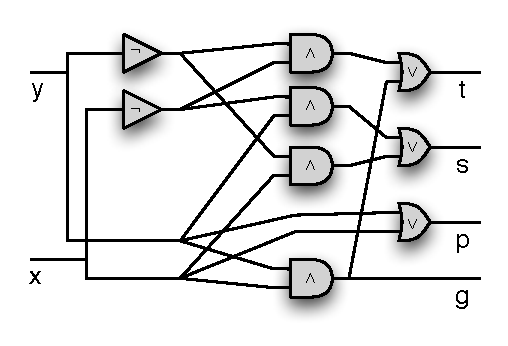
\includegraphics[height= 3cm ]{figs/DC1.pdf}
  \end{center}
  \column{0.5\linewidth}
  \begin{center}
    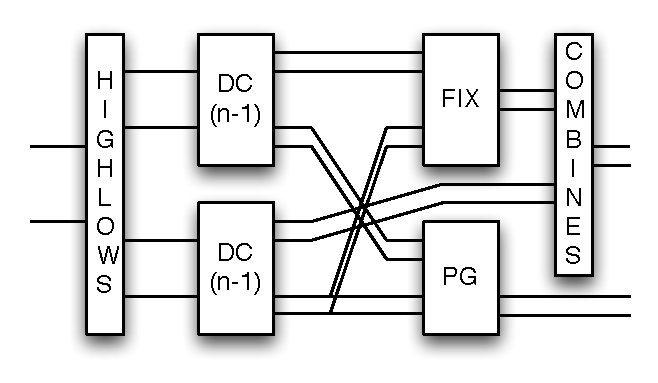
\includegraphics[height= 3cm ]{figs/DC.pdf}
  \end{center}
\end{columns}
\begin{columns}
\column{0.1\linewidth}
\column{0.5\linewidth}
\begin{scoq}
Variable V : T -> Type. 

Fixpoint add $\Phi$ n (x : V (Tint [2^ n])) (y : V (Tint [2^ n])) := 
match n  with 
| 0 => Return ( (x = 1) || (y = 1) ;
          (x = 1) && (y = 1); x + y; x + y + 1)




$$
\end{scoq}
\column{0.5\linewidth}
\begin{scoq}
| S n => 
  DO (xL,xH) <- (low x, high x);
  DO (yL,yH) <- (low y, high y);
  DO (pL, gL, sL, tL) <- add n xL yL; 
  DO (pH, gH, sH, tH) <- add n xH yH; 
  DO sH' <- (gL ? tH : sH);
  DO tH' <- (pL ? tH : sH);
  DO pH' <- (gH || (pH && gH));
  DO gH' <- (gH || (pH && gL));
  Return (pH'; gH'; sL $\otimes$ sH' ; tL $\otimes$ tH' )
end.  
\end{scoq}
\end{columns}
\parenthesis{builds a 4-uple: carry-propagate, carry-generate, sum w/ carry, sum w/o carry}
\end{frame}

\begin{frame}[fragile]
  \frametitle{Processor designs}
  \begin{itemize}
  \item Easy translation from old Bluespec papers
    \begin{columns}
\column{0.1 \linewidth}
\column{0.3\linewidth}
      \begin{coq}
Definition bz :=
DO pc <- ! PC 
DO I   <- IMEM.[pc] ; 
WHEN (opcode I =  3 );
DO r1 <- RF.[r1 I];
DO r2 <- RF.[r2 I];
If  r1 = 0 { PC := r2 }
Else {PC := pc + 1}
\end{coq}


\column{0.5\linewidth}
\begin{coq}
(** Rule BZ taken **)
Proc(PC,RF,IMEM,DMEM) 
if (RF[r1] = 0) where BZ(r1,r2) = IMEM[PC]
-> Proc(RF[r2],RF,IMEM,DMEM)

(** Rule BZ not taken **)
Proc(PC,RF,IMEM,DMEM) 
if (RF[r1] <> 0) where BZ(r1,r2) = IMEM[PC]
-> Proc(PC + 1,RF,IMEM,DMEM)
\end{coq}
\end{columns}

\item \coqe{Definition isa := loadi $\oplus$ loadpc $\oplus$  add $\oplus$ bz $\oplus$ load $\oplus$ store}
% \item Use a mixture of notations and intermediate definitions
\end{itemize}
\parenthesis{Not yet tried to prove anything about this one}
\end{frame}
%%%%%%%%%%%%%%%%%%%%%%%%%%%%%%%%%%%%%% 
\begin{frame}[fragile]
  \frametitle{PHOAS in action (2)}

  \begin{itemize}
  \item<1-> PHOAS shines when defining examples of circuits inside Coq: 
    \begin{itemize}
    \item makes it possible to use fancy coq notations 
\begin{coq}
Notation "'DO' X <- A ; B" := (Bind A (fun X => B)) ( ... )      
\end{coq}
\item other solutions (e.g., dependently typed de Bruijn indices) would not scale
\item keep all the benefits of deep-embeddings!
\end{itemize}
\end{itemize}
\end{frame}
%%%%%%%%%%%%%%%%%%%%%%%%%%%%%%%%%%%%%% 


\section{Conclusion}
% Rant about Coq
\begin{frame}
  \frametitle{Outline}       
  \tableofcontents [currentsection] 
\end{frame}

\begin{frame}[fragile]
  \frametitle{Some remarks}
  \begin{itemize}

  \item Stepping back
    \begin{itemize}
    \item Bluespec started as an HDL deeply embedded in Haskell
    \item Lava [1998] is another HDL deeply embedded in Haskell
    \item \fesi{} is ``just'' another HDL,  deeply embedded in \alert{Coq}
      \pause
      \begin{itemize}
      \item semantics (i.e., interpreter), compiler and programs are \alert{integrated seamlessly}
      \item use of computation \alert{inside} Coq to dump compiled programs
      \item dependent types capture some interesting properties in hardware
      \end{itemize}
    \end{itemize}

\pause

  \item Future work
      \begin{itemize}
      \item Improve on the language (inputs, FIFOs, schedulers)
      \item Better compiler (boolean optimisations/BDDs)
      \item Extraction/plugin to output actual VHDL/Verilog
      \item Prove some designs correct  
      \end{itemize}
      
\pause

    \item Closing remarks (wish-list)
      \begin{itemize}
      \item Generated induction principles useless
      \item Mutual fixpoints and inner fixpoints being not equivalent
      \item Could really use some help from SMT solvers to solve bitvector arithmetic goals
      \end{itemize}
  
    \end{itemize}
\end{frame}

\begin{frame}
  \frametitle{Thank you for your attention}
  
  \begin{center}
    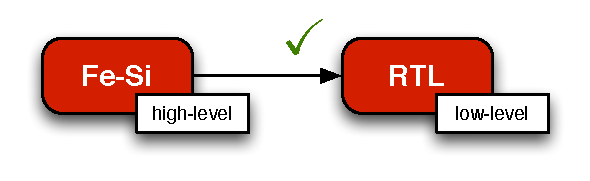
\includegraphics[height= 2cm ]{figs/compilation.pdf}

    \vspace{1cm}

    If you have any questions ... \\
  \end{center}
  
\end{frame}
\end{document}
